\section{Background}
\subsection{BrainScaleS-2}
\subsection{Host - HICANN-X Communication}
\begin{figure}
\centerline{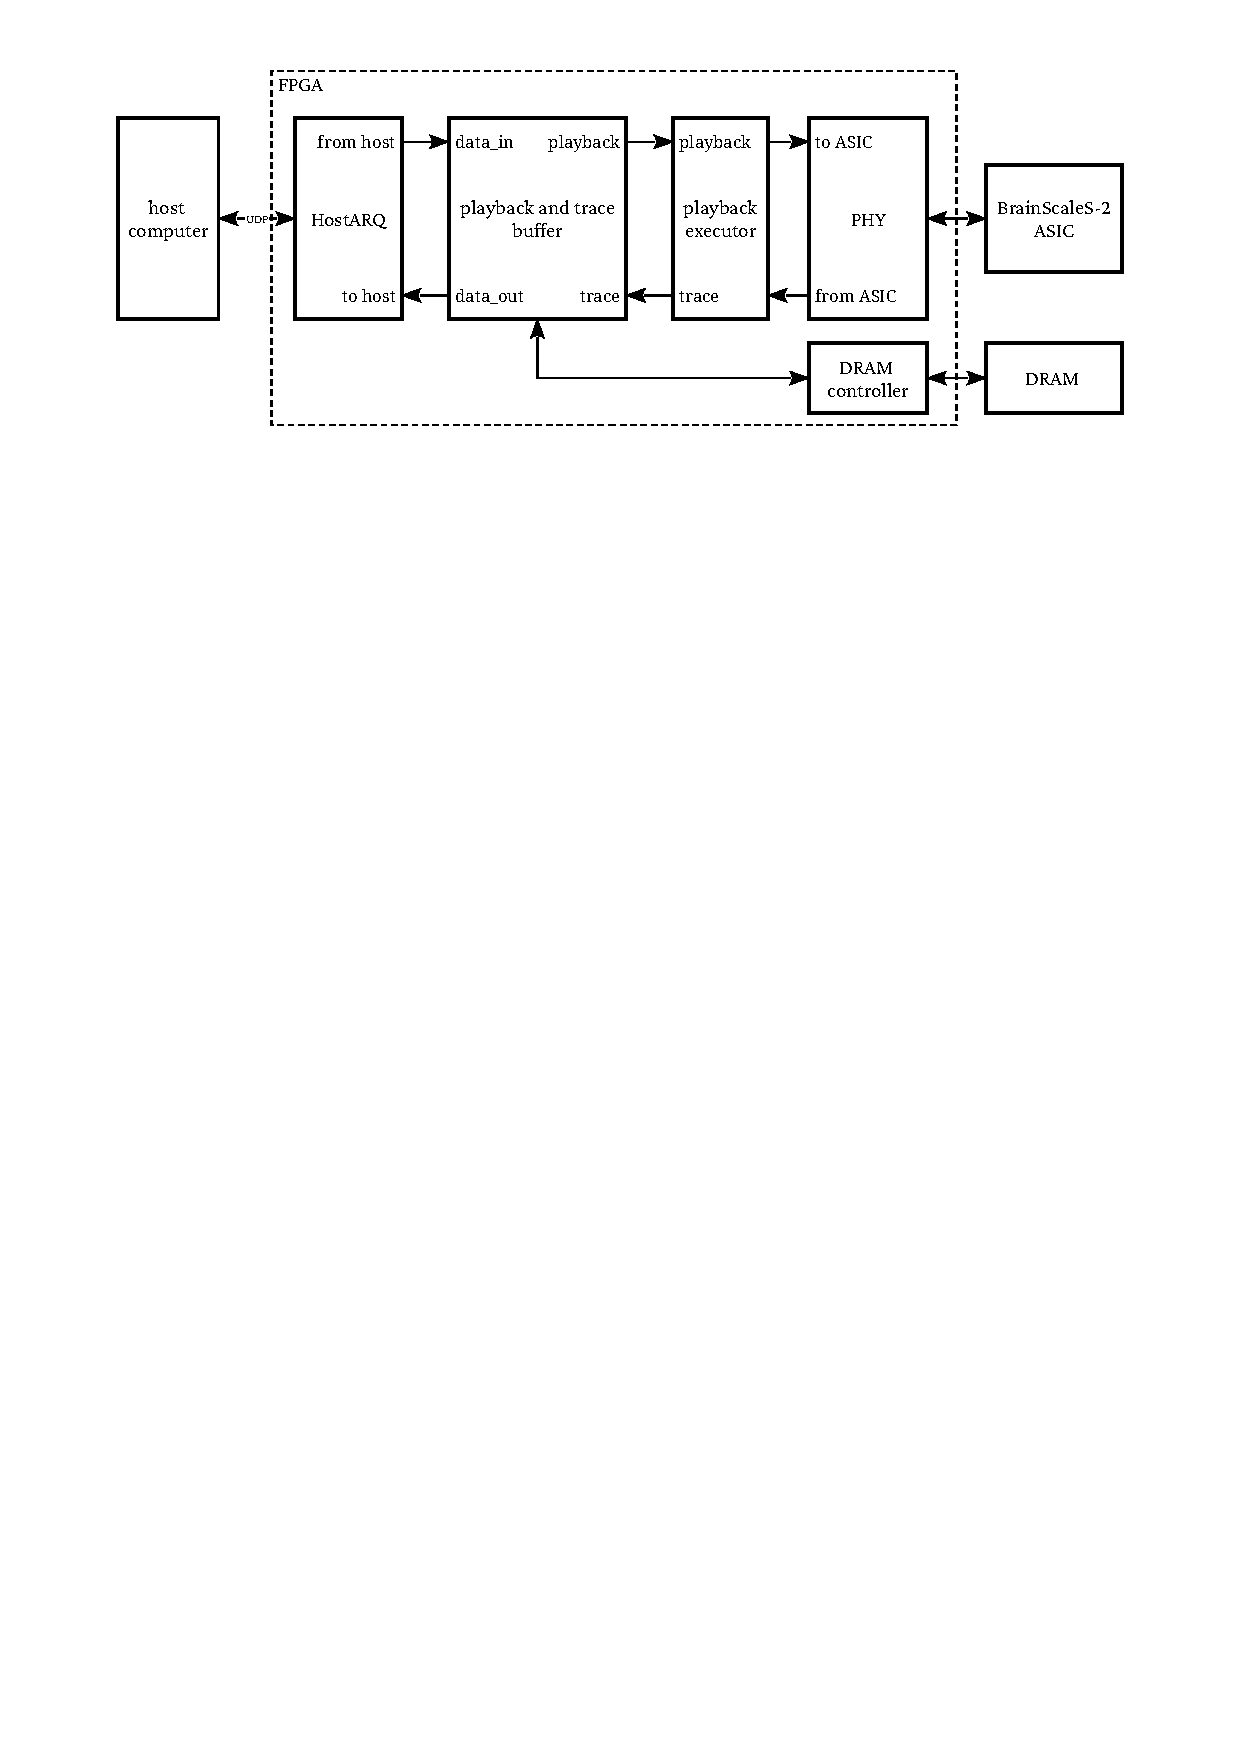
\includegraphics{diagrams/cropped/fpga_overview}}
\caption{Schematic overview of the FPGA design facilitating the communication between a network attached host computer and a HICANN ASIC}
\end{figure}

Communication with the \ASIC{} requires precise timing due to its physical nature, its emulation cannot be paused and resumed arbitrarily and a high data rate.
The high data rate interface of the \ASIC{} consists of eight pairs of \LVDS{} lanes, that can each operate at up to $\SI{2}{\giga\bit\per\second}$, for a total of $\SI{16}{\giga\bit\per\second}$ full duplex bandwidth.
To achieve the required precise timing a \FPGA{} is used to facilitate the communication between the host and the \ASIC{}.
Interaction with the \ASIC{} is converted into a sequence of instructions, the \PlaybackProgram{} that are processed by the \FPGA{} with deterministic timing at a resolution of $\SI{8}{\nano\second}$.
Data received from the \ASIC{} is timestamped with the same resolution by the \FPGA{}.

In the \BSSTwo{} system a \Xilinx{} \Kintex7{} \FPGA{} is used and the \LVDS{} lanes of the \ASIC{} are operated at $\SI{1}{\giga\bit\per\second}$.

The host and the \FPGA{} communicate using \UDP{} protocol over \Gigabitethernet{}. On top of \UDP{} the \HostARQ{}\autocite{ref:hostarq} protocol is used to implement a secured stream with a word size of \PhyWordSize{} over the unsecure \UDP{} protocol.

\subsubsection{Stream-Interfaces}
Many components of the \FPGA{} design are connected using stream interfaces. Throughout this thesis two different stream interfaces will be encountered. The first is \AXIStream{}\autocite{ref:axi_stream}, a standard interface used by many components provided \Xilinx{}.
\AXIStream{} is a unidirectional data stream, that connects a single master with a single slave. A \AXIStream{} consists of at least five signals:
\begin{itemize}
    \item \ACLK{} is the clock signal used by the stream. All other signals will be sampled on the rising edge of this clock.
    \item \ARESETn{} is the reset signal used by the stream. It is active low.
    \item \TDATA{} is the signal carrying the data. It is a multiple of eight bits wide and driven by the stream master.
    \item \TVALID{} is a single bit signal driven by the master indicating that valid data is present on the \TDATA{} signal.
    \item \TREADY{} is a single bit signal driven by the slave indicating that it can accept data.
\end{itemize}
The relation of \TDATA{}, \TVALID{} and \TREADY{} is governed by a set of rules. Data is transferred from the master to the slave when \TREADY{} and \TVALID{} are driven high simultaneously. This is called a two-way handshake mechanism.
Furthermore a master is not allow to wait for the slave to drive \TREADY{} high before asserting \TVALID{}. On the other hand, a slave is allowed to wait until the master drives \TVALID{} high until it drives \TREADY{} high.
When both the master and the slave can process the data fast enough, data can be transferred on every clock cycle. When this is the case \TREADY{} and \TVALID{} will be driven high continuously.
\AXIStream{} defines a set of further signals that can extend the functionality of this stream interface. In this thesis two optional signals will be relevant.
The first is \TKEEP{}. \TKEEP{} has one bit for every eight bits contained in the \TDATA{} signal and is driven by the master to indicate which bytes of the \TDATA{} signal contain valid data.
If bit $n$ of \TKEEP{} is driven high, bits $8n$ to $8(n + 1) - 1$ of \TDATA{} will contain valid data, if it is driven low the data contained in these bits is to be ignored by the slave.
The second optional signal is \TLAST{}. This is a single bit that is driven by the master which indicates that the current transfer is the last transfer of a packet.

The second stream type encountered in this thesis will be called \ValidNextStream{}. It is closely related to \AXIStream{}, but replaces the \TREADY{} signal with a \NEXT{} signal.
This is a single bit signal driven by the slave to indicate that the current data was processed and the master can present the next data word on \TDATA{}. Furthermore it has different rules regarding \TVALID{} and \NEXT{} compared to the rules of regarding \TVALID{} and \TREADY{}.
For a \ValidNextStream{} the master is allowed to wait until the slave drives \NEXT{} high before asserting \TVALID{}.

This different rule set means that in general a \AXIStream{} and a \ValidNextStream{} cannot be connected together by simply connecting the \TREADY{} and the \NEXT{} signals as they can deadlock. For example when connecting a \ValidNextStream{} master to a \AXIStream{} slave, the \ValidNextStream{} master is allowed to wait until the \AXIStream{} slave drives \TREADY{} (connected to \NEXT{}) until it drives \TVALID{}. However the \AXIStream{} slave is allowed to wait until \TVALID{} is driven high before asserting \TREADY{}. In this case both the slave and the master will wait forever and no progress will be made. This means when connecting a \ValidNextStream{} master to a \AXIStream{} slave, one has to use a \AXIStream{} slave that will assert \TREADY{} without waiting until \TVALID{} is asserted by the master.

\subsubsection{AXI}

\AXI{}\autocite{ref:axi} is standard communication bus used to connect some components of the \FPGA{} design. It is used to connect a single master to a single slave and is consists of a \ACLK{} and a \ARESETn{} signal that play the same role as they do in a \AXIStream{} as well as five independent channels:
\begin{itemize}
  \item The \AW{} channel transmits information about a write from the master to the slave. This information contains the address, the number of words that will be written (the \burstsize{}).
  \item The \AR{} channel transmits information about a read from the master to the slave. This information contains the address, the number of words that should be read (the \burstsize{}).
  \item The \W{} channel transmits the data that is written from the master to the slave.
  \item The \R{} channel transmits the data that is read from the slave to the master.
  \item The \B{} channel transmits a response that contains the result of a write from the slave to the master
\end{itemize}
Each of these channels uses the same handshaking signals \READY{} and \VALID{} as well as rules as a \AXIStream{}. Furthermore the \W{} and \R{} channels use a \LAST{} signal to indicate the last word of a burst.
Every channel operates separately from each other. This means that for example the data to be written can be transmitted by the master on the \W{} channel before the address information is transmitted on the \AW{} channel. A master is also allowed to transmit a second read on the \AR{} channel before having received the answer to the first.
From this it follows that the maximum data rate supported by the bus specification is a single data word each clock cycle on both the read and the write channels. Of course the actually data rate depends on the master and the slave.


\subsubsection{Playback Executor}
The \pbexec{} is responsible for processing the instruction stream that is received from the playback and trace memory management block as swell as receiving, time stamping and sending of events the trace stream events from the \ASIC{}.

The instructions that are processed by the executor can broadly be categorized into the three different categories of \readCat{}, \writeCat{}, \waitCat{}. Instructions of the \readCat{} category perform read operations on the several buses connected to the \pbexec{} and result result in response data that is sent to the trace stream in addition to the events from the \ASIC{}. Instructions of the \writeCat{} category perform writes to theses buses and instructions of the \waitCat{} are used to pause the processing of the instruction stream until a specific event takes place. This can for example be the elapsing of a specific duration or the completion of a read.

A special instruction, the \haltInstr{} is used to delineate separate experiments from each other. The \haltInstr{} marks the end of a \PlaybackProgram{} and looped back to the trace data where it can be used to differentiate trace data belonging to different \PlaybackProgram{}s.

The \pbexec{} operating at a \pbExecClock{} clock rate and can at most process a single instruction every clock cycle, however not every instruction can be processed in a single clock cycle. Obvious examples include instructions of the \wait{} category which purposefully pause the processing of the instruction stream. Similar to the instruction stream the \pbexec{} can also emit at most a single trace word every clock cycle.

% The maximum size of a playback instruction is $\SI{64}{\bits}$ which means

Both the playback instruction stream and the trace data are fundamentally a stream of variable size words. For transmission and reception over the fixed width \HostARQ{} streams they are encoded using \UT{} encoding scheme\autocite{ref:ut}.

For the playback instruction stream this encoding is performed on the host and on the \FPGA{} the \pbexec{} decodes the instruction stream before processing it.
Likewise the trace data generated / received by the \pbexec{} is encoded by the \pbexec{} before being sent to the trace stream.

The encoding and decoding also operates at a \pbExecClock{} clock rate and can produce / consume at most one \PhyWordSize{} sized word per clock cycle.

This means the maximum data rate at which the playback stream can be processed and the maximum data rate that is sent on the trace stream is
\[\PhyWordSize{} \pbExecClock{} = \pbExecBandwidth{}\]

\todo{write about arbitration priority}
\begin{figure}
\centerline{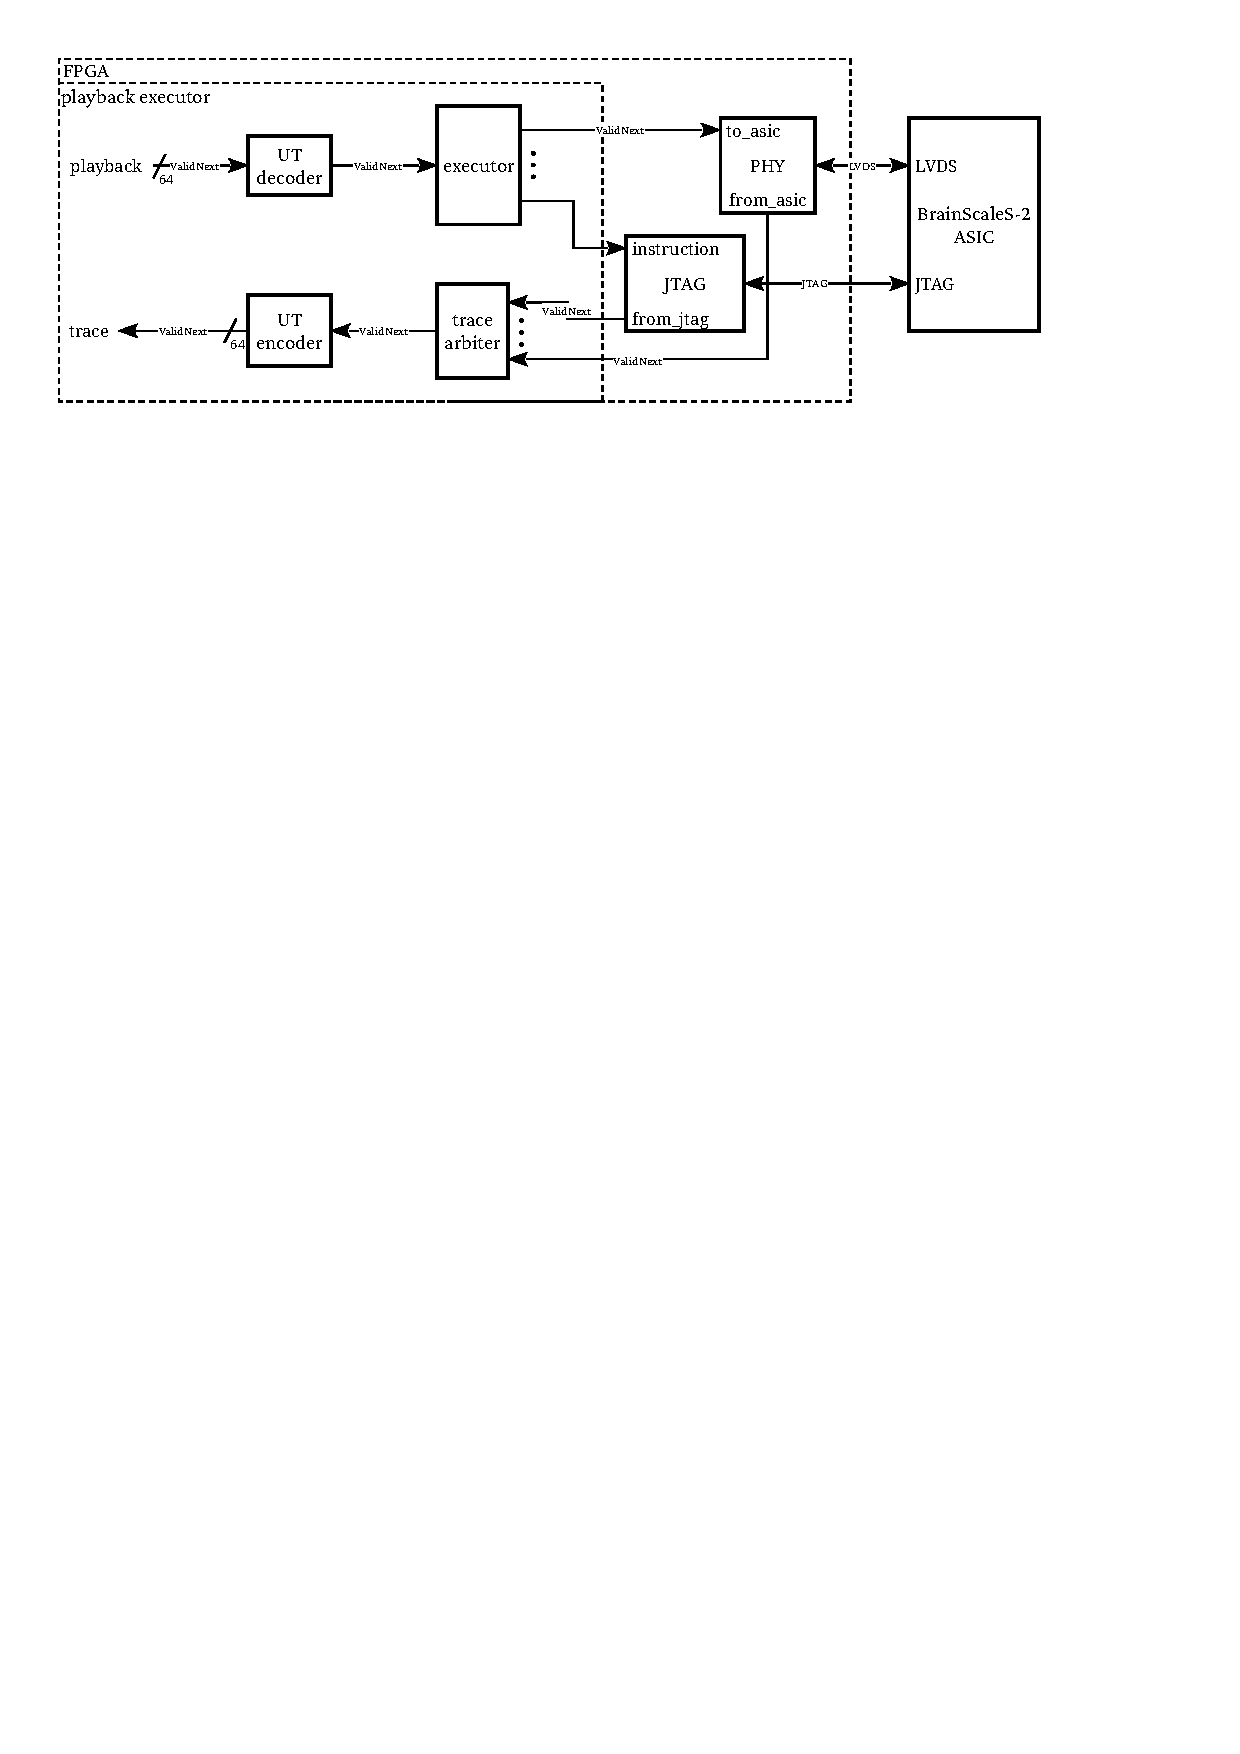
\includegraphics{diagrams/cropped/executor_detail}}
\caption{Overview of the \pbexec{}. This is on only a schematic representation and does not include all interfaces that the executor has access to and does not include all sources for trace data.}\label{diagram:executor}
\end{figure}

\subsubsection{Playback and Trace Memory Management}\label{sec:old-pb-trace-management}

The bandwidth between \FPGA{} and the \ASIC{} at \ASICBandwidth{} far exceeds the bandwidth between the host and the \FPGA{} of \HostBandwidth{}. To allow transmission and reception of the full data rate supported between the \FPGA{} and the \ASIC{} the \FPGA{} is connected to \SI{512}{\mebi\byte} of \DDR{} memory that is used as buffer for the playback and trace data. To interact with the \DDR{} memory the \XilinxMIG{} is used, configured to use a \AXI{} interface.

The playback and trace fifo management block responsible for storing the playback instructions stream received from the host into the \DDR{} memory and transmitting a complete experiment from the memory to the \pbexec{} as well as receiving the trace data from the \pbexec{} and storing it to the \DDR{} memory for later readout by the host.

In the current \FPGA{} design used by the \BSSTwo{} platform this block operates as a pair of \FIFO{}s. One for the playback stream and one for the trace stream. This \FIFO{} is implemented using the \Xilinx{} \VFIFO{} core, which implements a multi channel \FIFO{} backed by a \AXI{} accessible memory. It is connected to the \AXI{} interface of the \XilinxMIG{}. The \VFIFO{} core is used in a configuration using two channels. The first channel is used for the playback data and the second channel is used for the trace data.

The \pbmem{} block is responsible for scheduling the transmission of the playback instruction stream to the \pbexec{}.
It only allows data to be transmitted from the \VFIFO{} to the \pbexec{} when two conditions are fulfilled:
\begin{enumerate}
\item The \VFIFO{} channel for the playback data is empty or the \FIFO{} between the \VFIFO{} and the \pbexec{} is full
\item The \VFIFO{} channel for the playback data is full or a \haltInstr{} was written to the \VFIFO{} but not transmitted to the \pbexec{}
\end{enumerate}
When a complete \PlaybackProgram{} fits into the \VFIFO{} playback channel, these two conditions enforce that playback of the instructions that make up the \PlaybackProgram{} is only started once it was completely transmitted to the \VFIFO{}, as each \PlaybackProgram{} end with a \haltInstr{}. This ensures that the rate of instructions that can be transmitted to the \pbexec{} is not limited by the slow \HostARQ{} interface but instead by the \VFIFO{} and indirectly by the \XilinxMIG{} interface speed.
When a \PlaybackProgram{} does not fit completely in the \VFIFO{} playback channel, playback of it is started whenever the \VFIFO{} playback channel is full. This means that depending on rate the \pbexec{} is processing the playback instructions it is possible that the \HostARQ{} interface can be the limiting factor for the playback rate.
The \VFIFO{} is configured with a burst size of \(\SI{2048}{\byte}\) and using $\num{8192}$ $\SI{4}{\kibi\byte}$ allocated to each the playback and the trace channel, which means it can store at most \(\num{8192} · \SI{4}{\kibi\byte} = \SI{32}{\mebi\byte}\) per channel.

\begin{figure}
\centerline{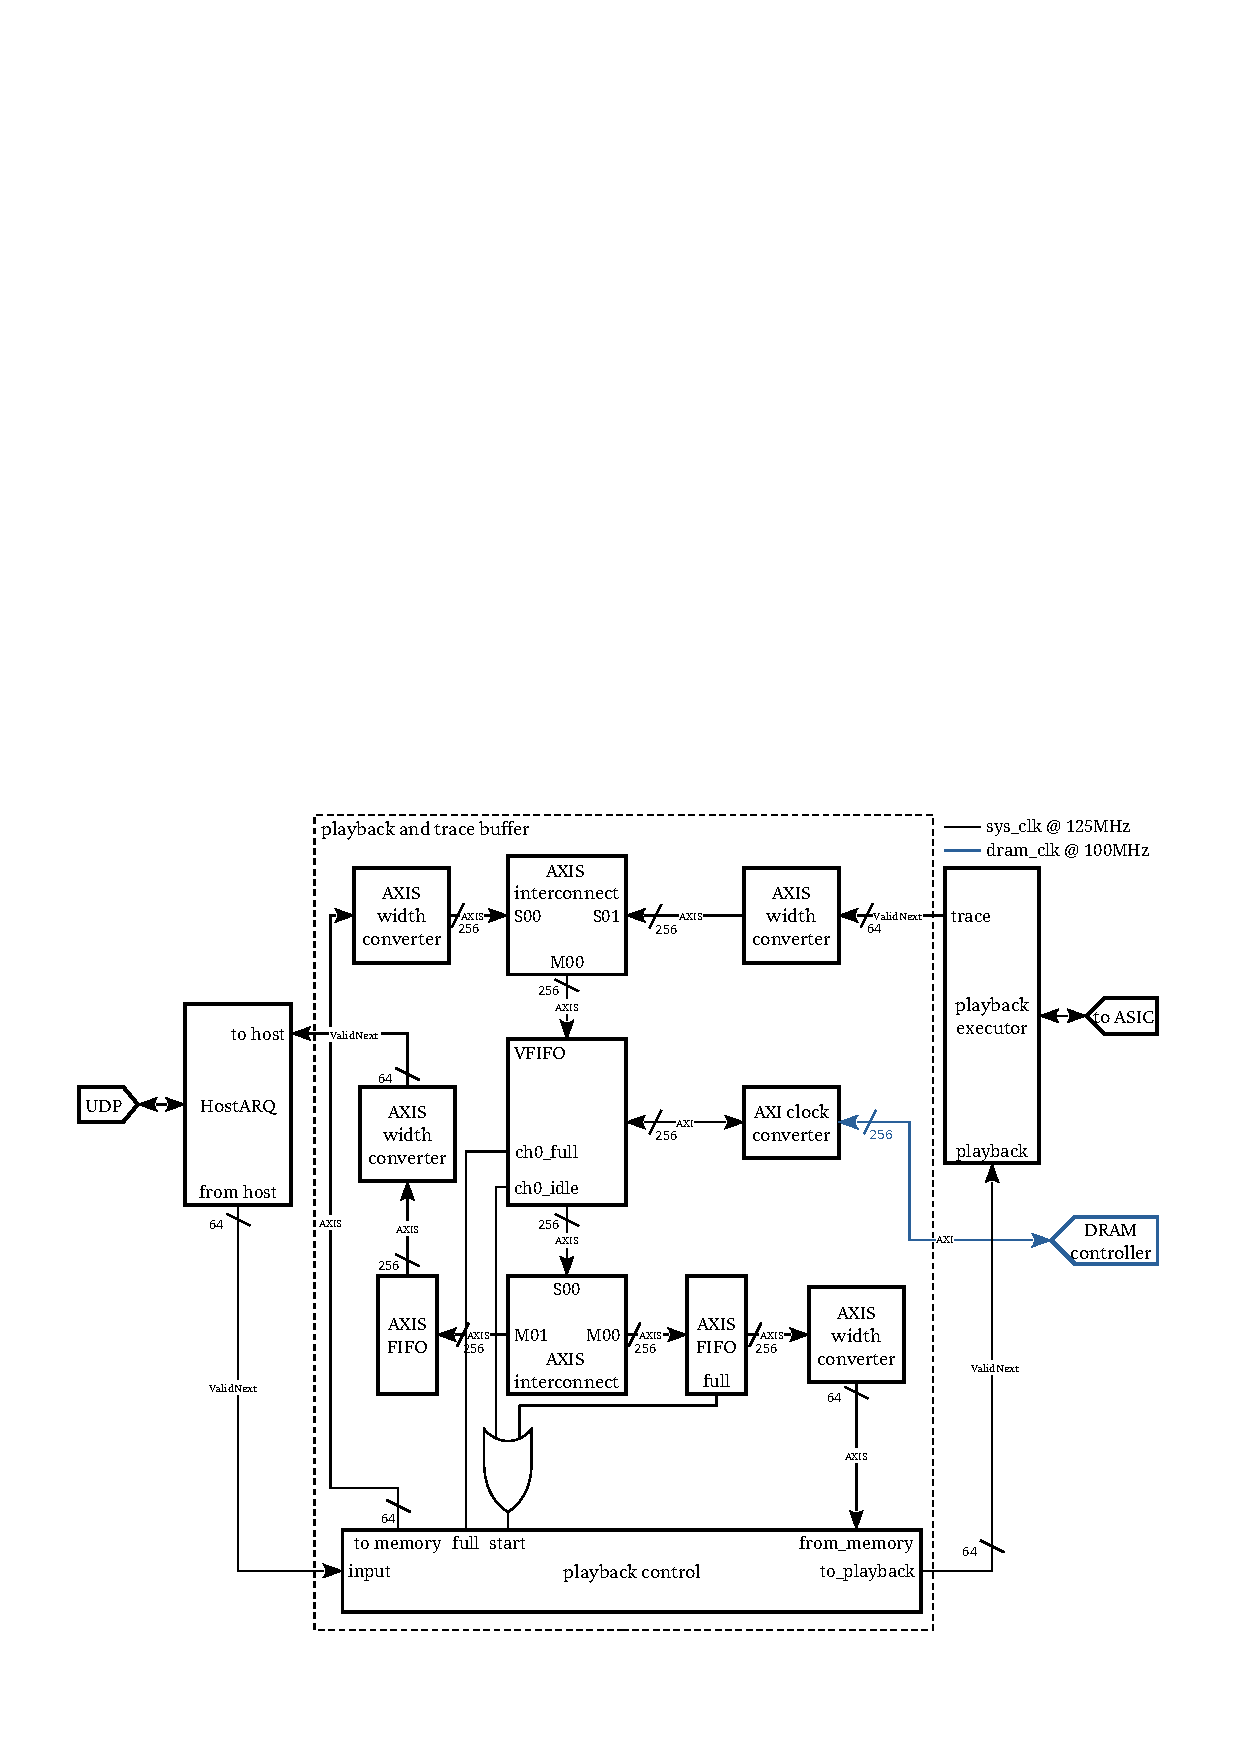
\includegraphics{diagrams/cropped/detail_old}}
\caption{Schematic overview of the old, FIFO-based, module handling the playback and trace data}\label{diagram:detail_old}
\end{figure}

This thesis will investigate a replacement for this \VFIFO{} based playback and trace memory management block.
